We validated our methodology by in a use-case concerning risk assessment for financial companies, inspired on the ORCA System\footnote{The ORCA System is a trademark of GCP Global www.gcpglobal.com.}.
Risk assessment is implemented by an interactive business process based on the exchange of a series of questionnaires intended to evaluate the risks implied the client's business practice.
For instance, the condition in which confidential transactions are performed, the physical security for accessing reserved areas (i.e. access to the critical servers room should be secured).
This information is used to determine whether there are risky actions within the business processes of the company that can be amended.
It is also used to determine a degree of compliance to existing norms.
By analysing the questionnaires, ORCA detects risky practices, proposes solutions and triggers further assessment processes to ensure that the solutions have been implemented.

Our goal is to model a service based application (called \textsl{FlyingPig}), for providing risk assessment as a service.
In order to provide this functionality \textsl{FlyingPig} would benefit from ORCA's legacy services: storage, assessment and data visualization functions.

In the following, we describe the results of applying $\Pi$-SODM to develop the \textsl{FlyingPig} risk assessment system.
The models presented next are the final results of the application of $\Pi$-SODM.
They were generated as a result of interactions with GCP Global software developers.

\begin{figure}
\centering
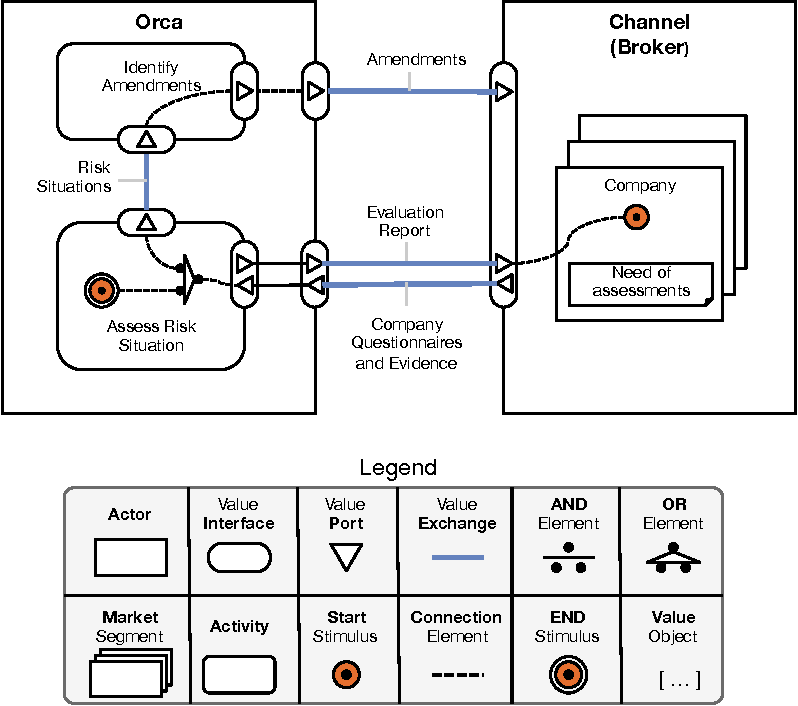
\includegraphics[width=0.7\textwidth]{figs/E3-Value.pdf}
\caption{E3value model of the FlyingPig.\label{fig:E3valuemodel}}
\end{figure}


\subsection{CIM}

$\Pi$-SODM uses two models, to be built at the CIM level (See Section~\ref{sec:modelingWithPISODM}).

Figure~\ref{fig:E3valuemodel} shows the value model~\cite{e3value} for the case of \textsl{FlyingPig}.
The value model is a business model that represents a business case graphically as a set of value exchanges ($\bigtriangleup\ \bigtriangledown$) and value activities (rounded boxes) performed by business actors (squared boxes).

In our use-case, we identify two business actors: \textsl{ORCA} and \textsl{Broker}. Brokers are the responsible for channeling requests for risk assessment of one or several companies. ORCA have two value activities which are services that provide it an economical benefit: to \textsl{identify amendments} and the possibility to \textsl{asses risk situation}. The value exchanged between ORCA and Brokers are: \textsl{amendments} and \textsl{evaluation reports} which are value objects ([...]) for the any companies that need to have a risk assessment, and the \textsl{questionnaire and evidences} and the risk assessment \textsl{fee} which are value objects for ORCA System.

Beside the static representation of a business case, the value model allows for the representation of dependency paths which enhance the understanding of a business idea by showing all value exchanges triggered by the occurrence of an end-consumer need. A dependency path has a direction and consists of dependency nodes linked by mean of connections. A dependency node is a start stimulus, an AND-fork or AND-join, an OR-fork or OR-join, or an end node (see Legend on Figure~\ref{fig:E3valuemodel}). An start stimulus represents a trigger for the exchange of economic value objects while an end node represents a model boundary.

Figure~\ref{fig:E3valuemodel} shows the dependency paths for \textsl{FlyingPig}. The dependency path identified in that case is the need of assessment of a particular company. It denotes a stimulus caused by the client company who ask for risk assessment. Once this need occurs the value exchanges between ORCA and Broker are triggered. The value model represent that ORCA will provide amendments and an evaluation report in return for the questionnaire and evidences and the fees provided by the Broker. 

{\color{blue} Javier: Please modify the value model to include fee as a value object in return for evaluation report. Modified figure is on the git}

A better understanding of the process in which these value exchanges occurs may be modeled using a BPMN model. Figure~\ref{fig:bpmn} shows the BPMN model\footnote{Details on BPMN (Business Process Management Notation) can be found in http://www.bpmn.org/} for the scenario. It includes two pools representing the \textsl{ORCA} system and the \textsl{Brokers}. Brokers have two lanes, the client \textsl{Company} and a \textsl{User}. The user is a contact member of the company, who will coordinate the assessment process. This process will involve other members of the company as well.

The process starts by a request from a company asking for a risk assessment. Note that it is in agreement with the explanation of the start stimulus on the value model above. The request leads to the definition of a group of users that will answer questionnaires for evaluating risk. Questionnaires are considered tasks that users will have to perform. Given a list of tasks, the company assign a responsible and delegate the task. A task may be to answer a questionnaire or add an evidence but also could implies to solve some "risky situation" (e.g. to repair a door {\color{blue} ...¿Genoveva mira por favor si esto puede ser o hay algun ejemplo mas bueno/serio???} ).

Once a tasks are completed they are stored and analyzed to generate a set of un-compliant situations associated to their corresponding amendments if there are any or a report specifying a compliance level, incidents and a risk map.
During the process of analysing a questionnaire, the answers of some questions can trigger the generation of other questionnaires or amendments, that become new tasks to be executed.  

Business processes have also associated rules and constraints that define their non functional requirements.
NFR represents the ``semantics'' and the conditions in which the tasks must be done.
In our example we have some constraints.
\begin{itemize}
\item {\color{magenta} Placido and Umberto: Could you please complete these items? --G \& M.}
\end{itemize}

\begin{figure}[t]
\centering
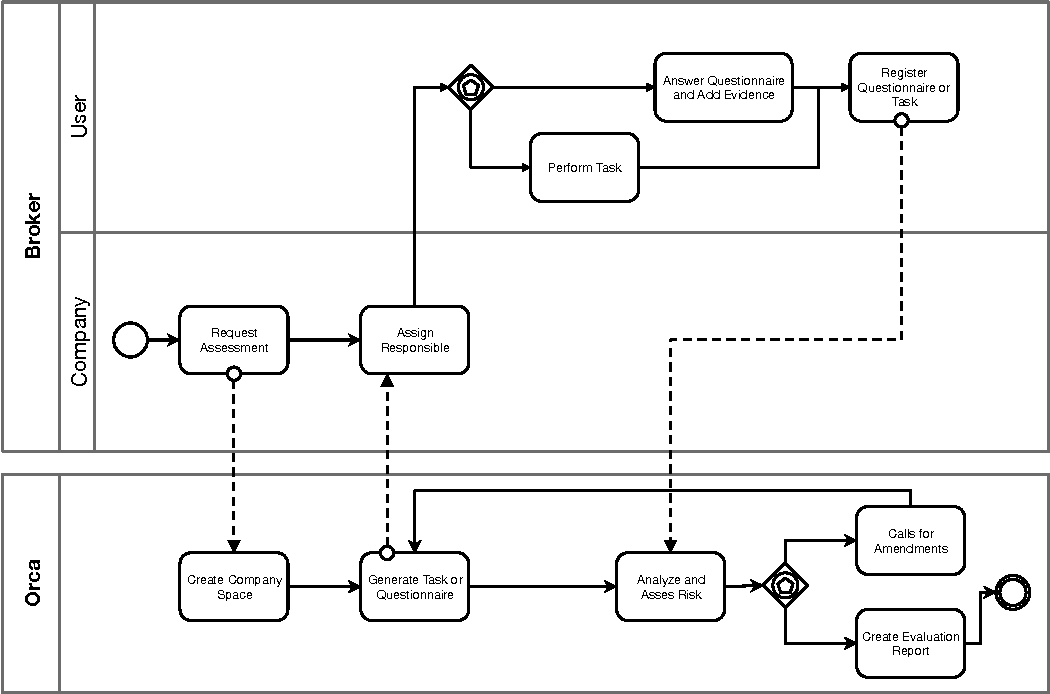
\includegraphics[width=1.0\textwidth]{figs/BPMN_GCP.pdf}
\caption{BPMN model for FlyingPig.\label{fig:BPMNmodel}}
\label{fig:bpmn}
\end{figure}


\subsection{PIM}


{\color{magenta} Placido and Umberto: Could you please comment models here? --G \& M.}


\begin{figure}
\centering
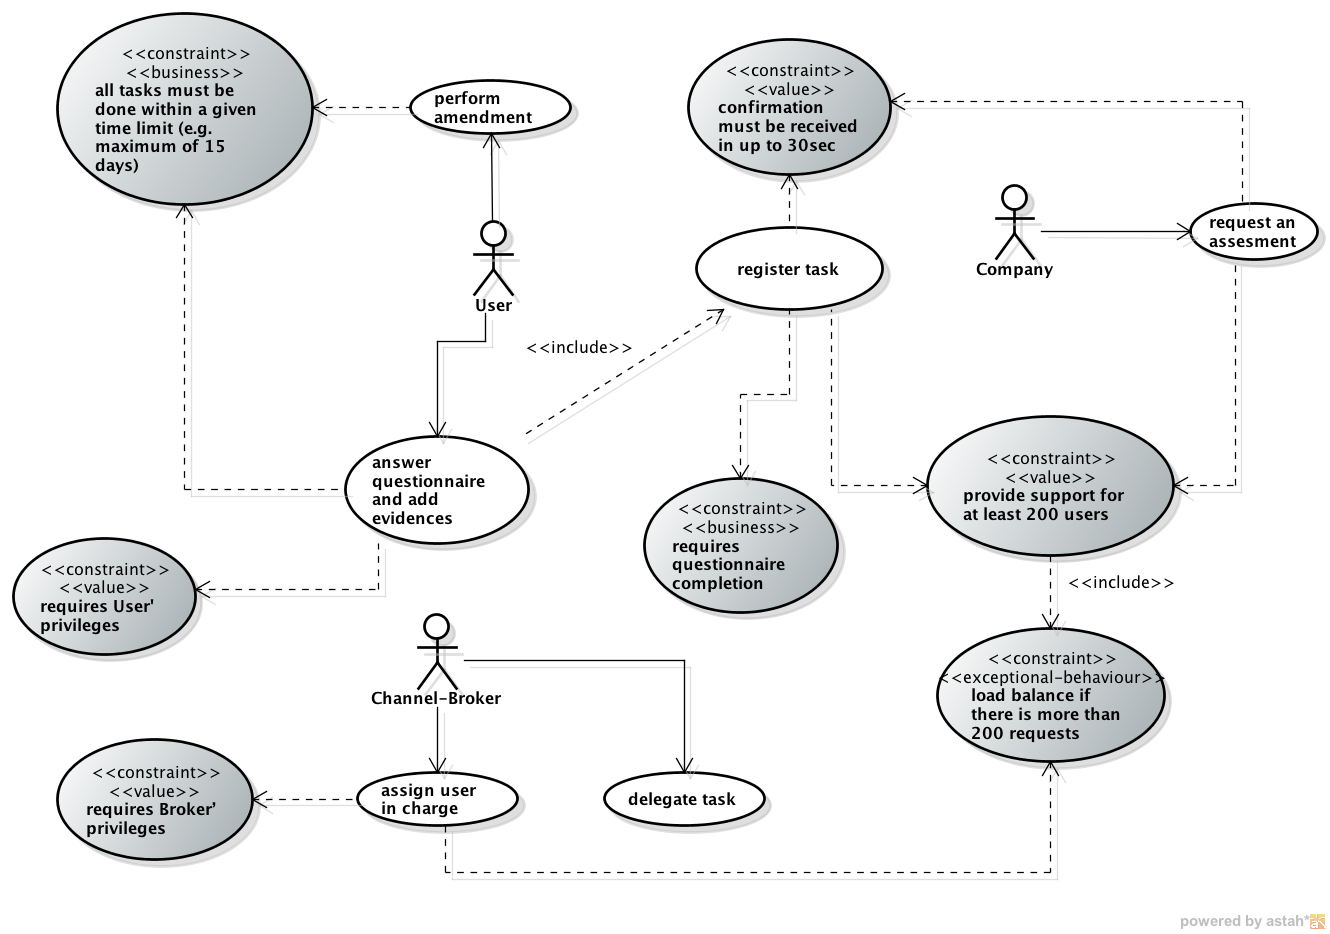
\includegraphics[width=1.0\textwidth]{figs/UseCaseGeneral.png}
\caption{$\pi$-UseCase model for FlyingPig.\label{fig:piUseCaseModel}}
\label{fig:bpmn}
\end{figure}

\begin{figure}
\centering
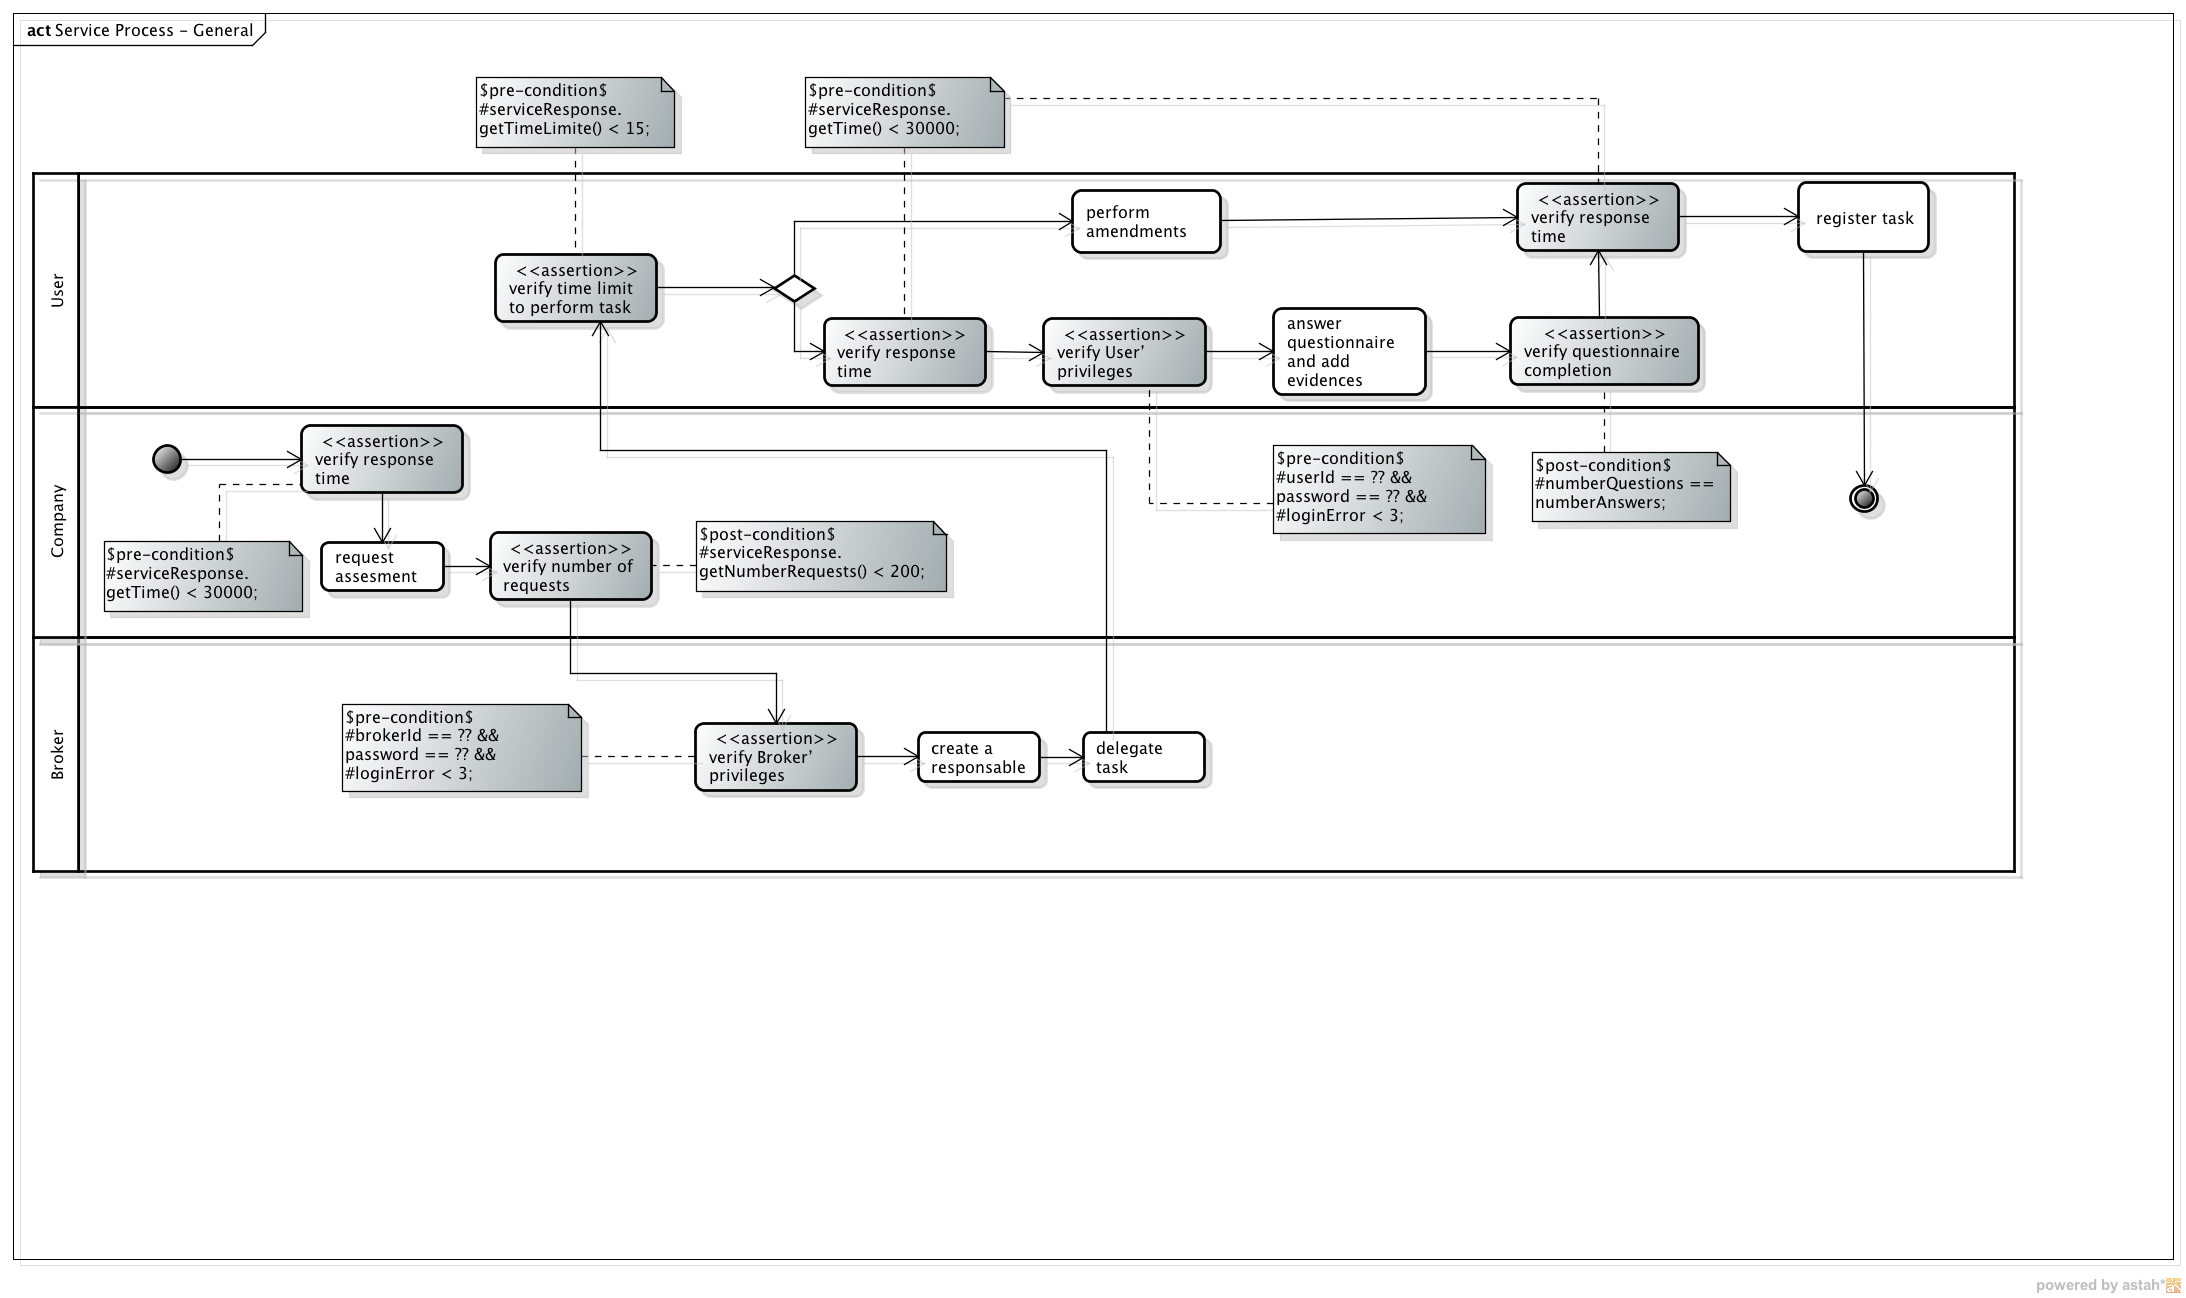
\includegraphics[width=1.0\textwidth]{figs/ServiceProcessGeneral.png}
\caption{$\pi$-ServiceProcess model for FlyingPig.\label{fig:PiServiceProcessModel}}
\label{fig:bpmn}
\end{figure}

\begin{figure}
\centering
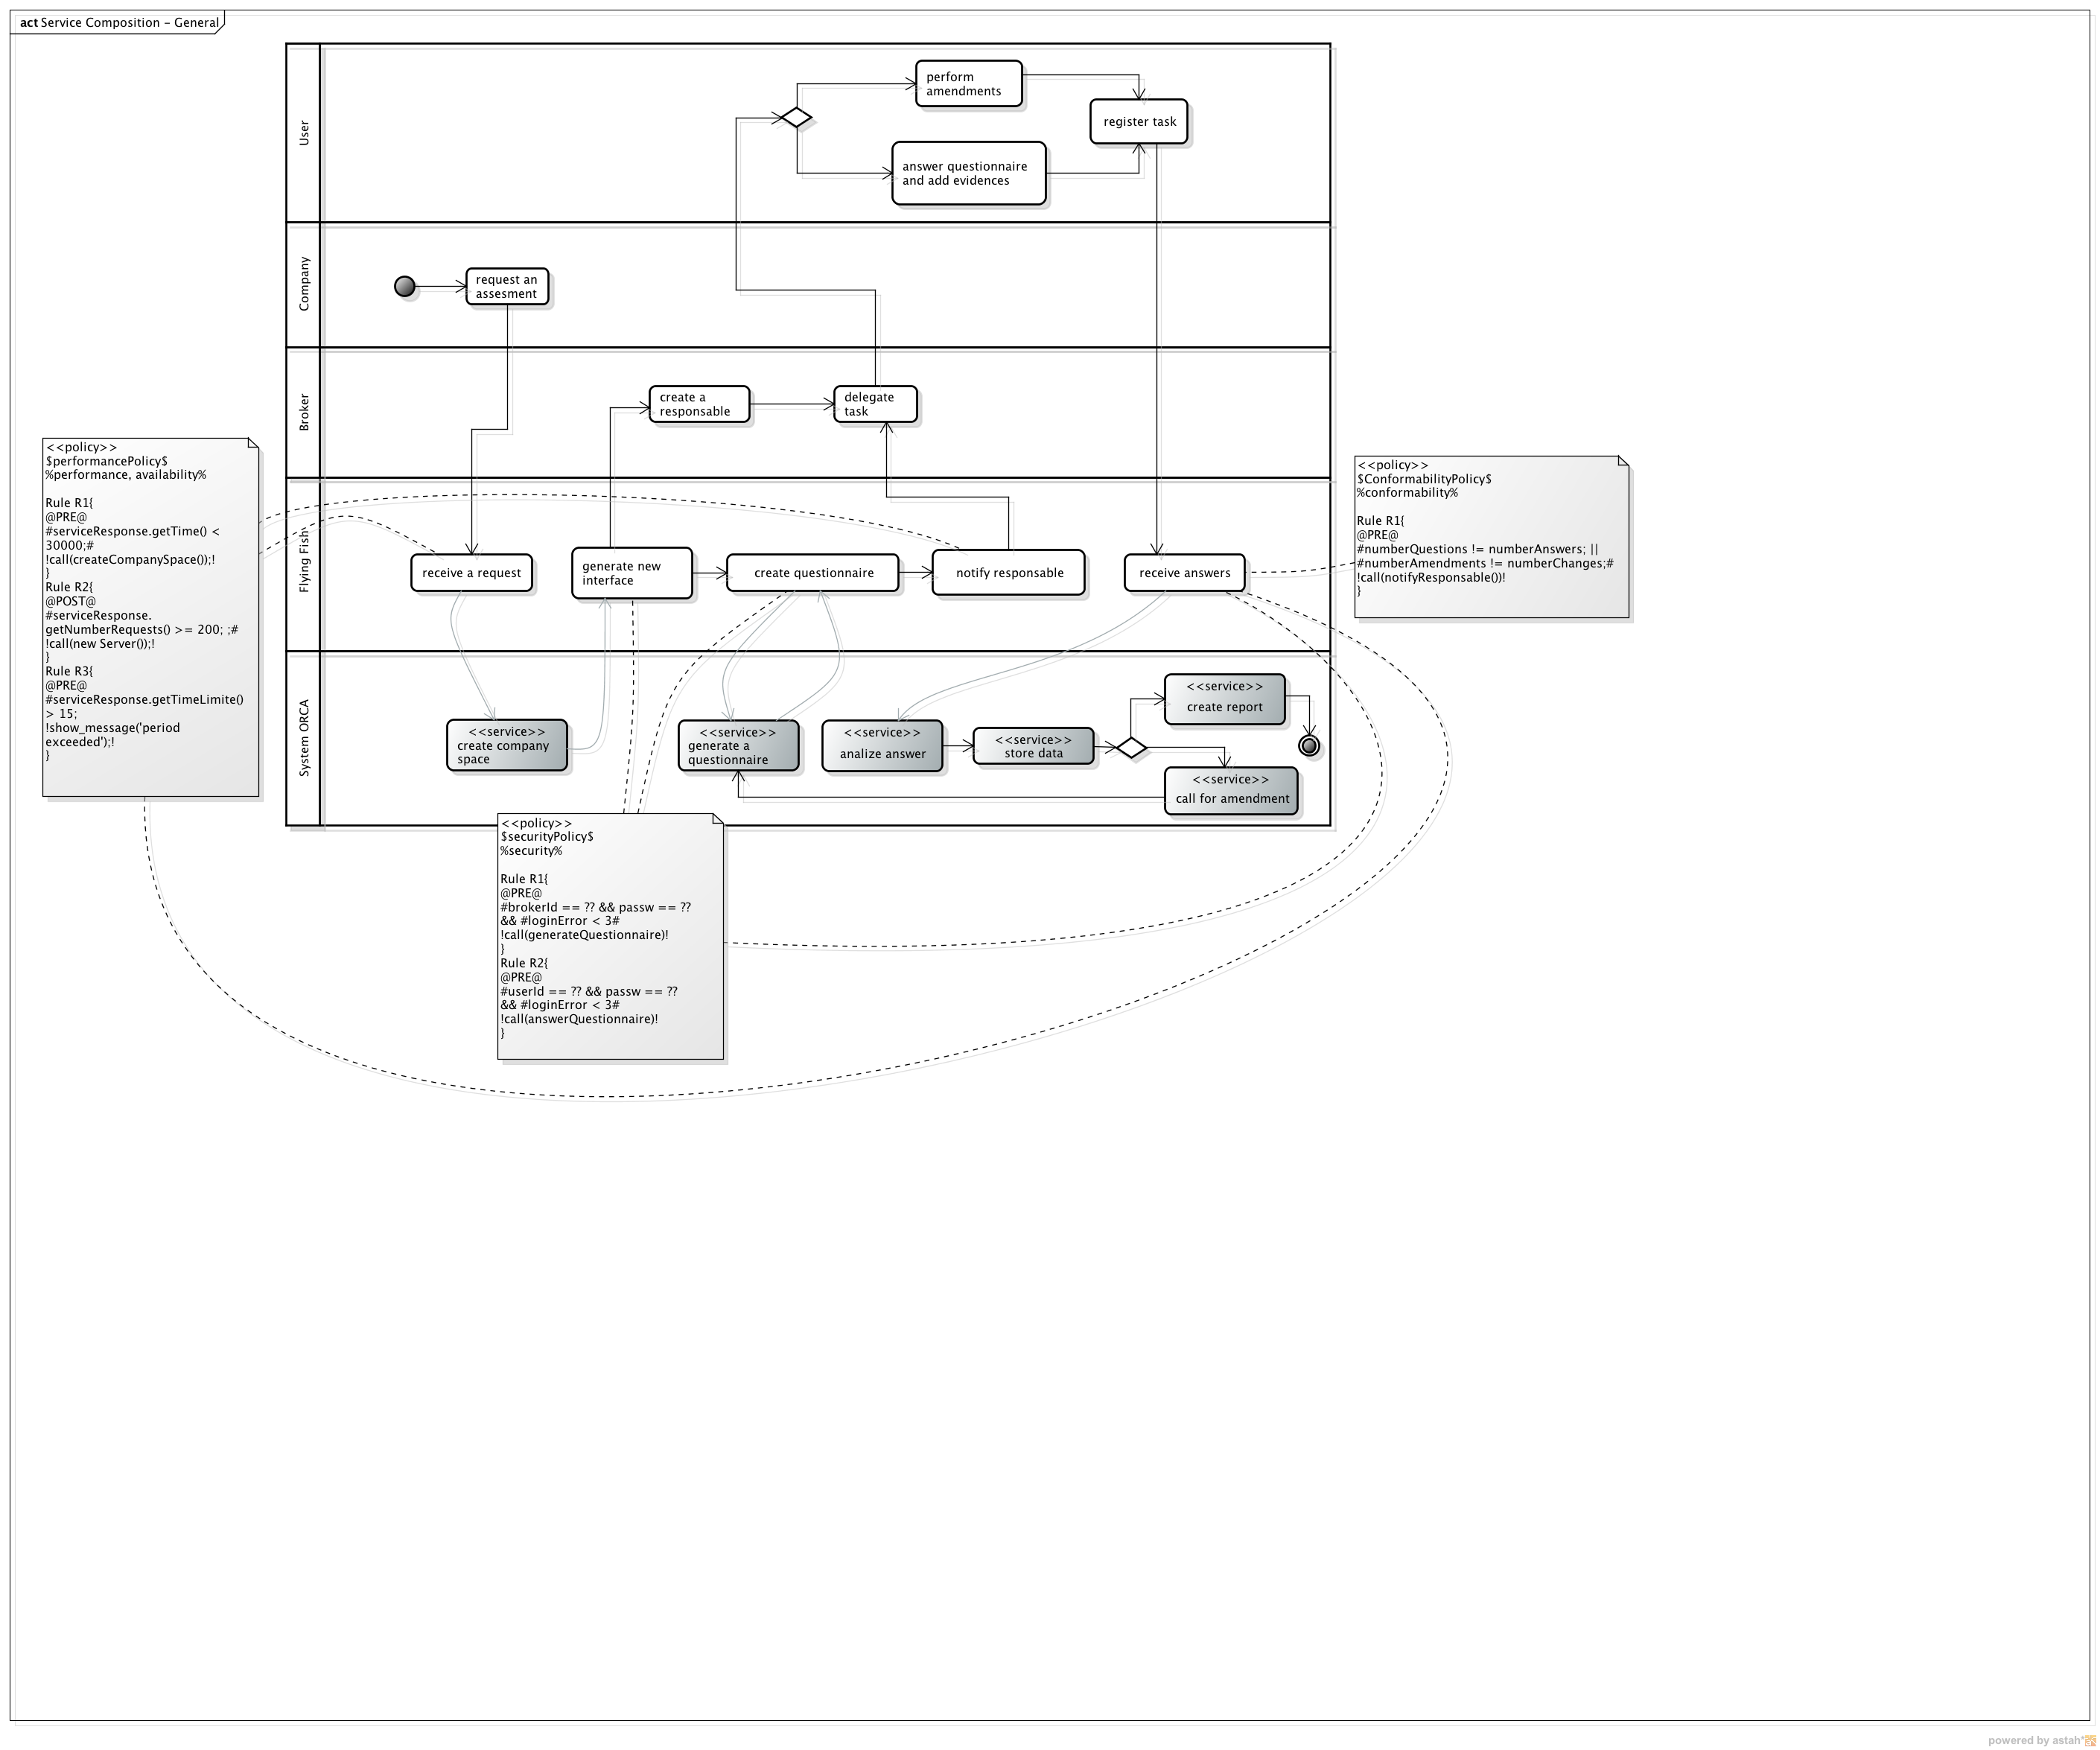
\includegraphics[width=1.0\textwidth]{figs/ServiceCompositionGeneral.png}
\caption{$\pi$-ServiceComposition model for FlyingPig.\label{fig:PiServiceCompositionModel}}
\label{fig:bpmn}
\end{figure}


\subsection{PSM}

{\color{magenta} Placido and Umberto: Could you please insert the $\pi$-PEWS model here? --G \& M.}


\subsection{Lessons Learned}

Through the example we underlined that every application implements functional aspects that describe its application logic.
Recall that an application logic refers to routines that perform the activities to reach the application objective.
Also there are non functional properties derived from NFR. They refer to strategies to be considered for the application execution like: security, isolation, adaptability, atomicity, and more.
These non functional properties must be ensured at execution time, and they are not completely defined within the application logic.

The challenge is to define them and to associate them with the application logic considering that different to existing solutions that suppose that it is possible to access the execution stat of all the components  of an application and that the application has complete control on them, in the case for service oriented applications  the components are autonomous services
API does not necessarily export information about methods dependency (e.g., in the REST protocol);
they do not share their state (stateless).

Given a set of services with their exported methods known in advance or provided by a  service directory, building services' based applications can be  a simple task that implies expressing an application logic as a services' composition. The challenge being  ensuring the compliance between the specification and the resulting application. Software engineering methods (e.g., \cite{1,2,decastro1,PapazoglouH06}) today can help to ensure this compliance, particularly when information systems include several sometimes complex business processes calling Web services or legacy applications exported as services.
